\documentclass[a4paper,14pt]{extarticle}
\usepackage{../../tex-shared/report-layout}

\renewcommand{\mylabnumber}{2}
\renewcommand{\mylabtitle}{Исследование коллективного типа передачи данных, групп и коммуникаторов в MPI}
\renewcommand{\mysubject}{Теория распределенных систем и параллельных вычислений}
\renewcommand{\mylecturer}{Дрозин А. Ю.}

\begin{document}
\begin{titlepage}
    
    \thispagestyle{empty}
    
    \begin{center}
        
        Министерство науки и Высшего образования Российской Федерации \\
        Севастопольский государственный университет \\
        Кафедра ИС
        
        \vfill

        Отчет \\
        по лабораторной работе №\mylabnumber \\
        \enquote{\mylabtitle} \\
        по дисциплине \\
        \enquote{\MakeTextUppercase{\mysubject}}

    \end{center}

    \vspace{1cm}

    \noindent\hspace{7.5cm} Выполнил студент группы ИС/б-17-2-о \\
    \null\hspace{7.5cm} Горбенко К. Н. \\
    \null\hspace{7.5cm} Проверил \\
    \null\hspace{7.5cm} \mylecturer

    \vfill

    \begin{center}
        Севастополь \\
        \the\year{}
    \end{center}

\end{titlepage}

\section{Цель работы}
Исследовать способы обмена данными между процессами в режиме широковещания или
группового обмена с использованием MPI-функций.

\section{Постановка задачи}
Вариант №1. Реализовать блочный алгоритм распределенного параллельного
перемножения матриц $A$ и $B$ с размерами $(8 * 5)$ и $(5 * 3)$ соответственно.
Вид распределяемых между процессами блоков представлен на рисунке \ref{fig:task}.

\begin{figure}[H]
    \centering
    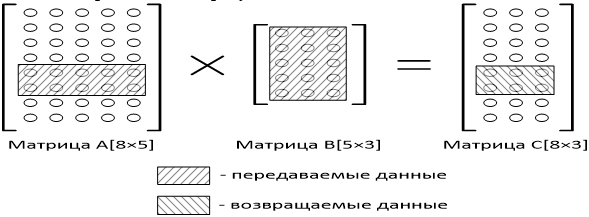
\includegraphics[width=.6\linewidth]{task}
    \caption{Перемножение матриц}
    \label{fig:task}
\end{figure}

\section{Ход работы}
Исходный код программы представлен на листинге:
\begin{lstlisting}
#include <iostream> 
#include <fstream> 
#include <mpi.h> 
#include <iomanip> 
  
using namespace std; 
  
int len_for_node(int size, int all) { 
    if (size == 1) { 
        return all; 
    } 
    if (!(all % size)) { 
        return all / size; 
    } 
    return 0; 
} 
  
void master() { 
    int size; 
    MPI_Comm_size(MPI_COMM_WORLD, &size); 
    if (size == 1) { 
        cout << "Can`t run without slaves! Just buy some..." << endl; 
        return; 
    } 
    ifstream is("input.txt"); 
    int n, k, m; 
    is >> n >> k >> m; 
    int *init_data = new int[4]; 
    init_data[0] = n; 
    init_data[1] = k; 
    init_data[2] = m; 
  
    int len = len_for_node(size - 1, n); 
    init_data[3] = len; 
    if (!len) { 
        cout << "Can`t split lines by processes" << endl; 
        exit(418); 
    } 
  
    MPI_Barrier(MPI_COMM_WORLD); 
    MPI_Bcast(init_data, 4, MPI_INTEGER, 0, MPI_COMM_WORLD); 
    delete[] init_data; 
  
    int *a = new int[n * k], 
            *b = new int[k * m]; 
    for (int i = 0; i < n * k; i++) { 
        is >> a[i]; 
    } 
    for (int i = 0; i < k * m; i++) { 
        is >> b[i]; 
    } 
  
    int *empty = new int[len * k]; 
    int *buf = new int[(len + n) * k]; 
    memcpy(buf + (len * k), a, n * k * sizeof(int)); 
  
    MPI_Barrier(MPI_COMM_WORLD); 
    MPI_Scatter(buf, len * k, MPI_INTEGER, empty, len * k, MPI_INTEGER, 0, MPI_COMM_WORLD); 
    delete[] empty; 
    delete[] buf; 
    delete[] a; 
  
    MPI_Barrier(MPI_COMM_WORLD); 
    MPI_Bcast(b, k * m, MPI_INTEGER, 0, MPI_COMM_WORLD); 
    delete[] b; 
  
    int *c = new int[(len + n) * m]; 
    empty = new int[len * m]; 
    MPI_Barrier(MPI_COMM_WORLD); 
    MPI_Gather(empty, len * m, MPI_INTEGER, c, len * m, MPI_INTEGER, 0, MPI_COMM_WORLD); 
  
    for (int i = 0; i < n; i++) { 
        for (int j = 0; j < m; j++) { 
            cout << setw(5) << c[len * m + i * m + j] << " "; 
        } 
        cout << endl; 
    } 
    delete[] c; 
} 
  
void slave() { 
    int *buf = new int[4]; 
  
    MPI_Barrier(MPI_COMM_WORLD); 
    MPI_Bcast(buf, 4, MPI_INTEGER, 0, MPI_COMM_WORLD); 
    int k = buf[1], 
            m = buf[2], 
            len = buf[3]; 
    delete[] buf; 
  
    int empty[0]; 
    int *a = new int[len * k]; 
  
    MPI_Barrier(MPI_COMM_WORLD); 
    MPI_Scatter(empty, 0, MPI_INTEGER, a, len * k, MPI_INTEGER, 0, MPI_COMM_WORLD); 
  
    int *b = new int[k * m]; 
  
    MPI_Barrier(MPI_COMM_WORLD); 
    MPI_Bcast(b, k * m, MPI_INTEGER, 0, MPI_COMM_WORLD); 
  
    int *c = new int[len * m]; 
    for (int i = 0; i < len; i++) { 
        for (int j = 0; j < m; j++) { 
            c[i * m + j] = 0; 
            for (int y = 0; y < k; y++) { 
                c[i * m + j] += a[i * k + y] * b[y * m + j]; 
            } 
        } 
    } 
    delete[] a; 
    delete[] b; 
  
    MPI_Barrier(MPI_COMM_WORLD); 
    MPI_Gather(c, len * m, MPI_INTEGER, empty, 0, MPI_INTEGER, 0, MPI_COMM_WORLD); 
    delete[] c; 
} 

int main(int argc, char **argv) { 
    int rank; 
  
    MPI_Init(&argc, &argv); 
    MPI_Comm_rank(MPI_COMM_WORLD, &rank); 
  
    rank ? slave() : master(); 
  
    MPI_Finalize(); 
    return 0; 
}
\end{lstlisting}

\section*{Выводы}
В ходе выполнения лабораторной работы были исследованы способы обмена данными
между процессами в режиме широковещания или группового обмена с использованием
MPI-функций. Написана программа умножения двух матриц произвольного размера,
распределяющая расчет строк динамически между кратным количеством процессов-рабочих.
\end{document}